\documentclass{article}
\usepackage{amsmath}
\usepackage{graphicx}
\usepackage{float}
\title{Homework 2}
\author{Bastian Haase}
\date{}
\begin{document}
\maketitle
\section{Exercise 1}
We will compare the performance of the steepest decent method to the quasi-Newton method in this
section. For the quasi-Newton method, we will use three different techniques to modify the
hessian if it is not positive definite.\par
The first technique that we will abbreviate with \emph{fcol} is the one described in Algorithm 3.3
in our textbook of Nocedal and Wright. The main idea is to add a small multiple of the identity to the hessian until choleski factorization works.\par
The second technique, \emph{spec},  analyzes the spectrum of the matrix. If the smallest eigenvalue $\lambda$ is negative,  we  multiply the identity with a scalar $|\lambda|+\epsilon$ for small $\epsilon$ and add this to our hessian.
We have chosen $\epsilon=10^{-3}$ for this comparison.\par
Lastly, instead of modifying the hessian, we just try to solve the resulting system of linear
equations with the conjugate gradient method, \emph{cg}. In case the hessian is not positive definite,
we still get an approximation of the solution of this system. \par
In all cases, we will determine the step length by use of a backtracking method starting with
a length of $1$ and dividing it by $2$ if the Wolfe condition is not satisfied.
\subsection{Setup and Parameters}
We are considering the Rosenbrock function
\begin{align*}
  f(x,y)=(1-x)^2+100(y-x^2)^2
\end{align*}
which attains its minimum at $(1,1)$. The following table lists the parameters we have chosen.
\begin{table}[H]
  \centering
  \begin{tabular}{|l|c|c|c|c|}
    \hline
   \textbf{Parameter} & Tolerance & Max Iterations & Max Iterations Step Size & $c_{1}$ \\ \hline
   \textbf{Value}     & $10^{-6}$   & $10^{5}$ & $10^{2}$ & $10^{-4}$ \\ \hline
  \end{tabular}
  \caption{Parameters for Comparison}
  \label{tab:param}
\end{table}
Here, \emph{Max Iterations Step Size} denotes the maximum number of modifications of our step length at each step
of our iteration.
We will compare all four methods with a starting point where the hessian is spd and at a point where it is not. Additionally, we will determine the region of convergence by applying all methods
to a $32 \times 32$ mesh of the set $[-2,2] \times [-1,3]$.

\subsection{Hessian spd}
We can see that the hessian of the Rosenbrock function at the point $(-1.9375,-0.9375)$ is positive
definite, as the eigenvalues are both positive. The  table illustrates the performance
of the four methods with this starting point and the setup described above.
\begin{table}[H]
  \centering
  \begin{tabular}{|l|c|c|c|}
    \hline
   \textbf{Method} & \textbf{Iterations} & \textbf{Function Evaluations} &\textbf{Jacobian Evaluations} \\ \hline
   steep &17914 &122537 &10001 \\ \hline
   fcol &25 &83 &26 \\ \hline
   spec &25 &83 &26 \\ \hline
   cg &25 &83 &26 \\ \hline
 \textbf{Method} & \textbf{Hessian Evaluations} & \textbf{Matrix Factorizations} & \textbf{Multiplications with Hessian} \\ \hline
 steep &0 & 0 & 0 \\ \hline
   fcol &25 &25 &25 \\ \hline
   spec &25 &50 &25 \\ \hline
   cg &25 &0 &50 \\ \hline
  \end{tabular}
  \caption{Performance SPD}
  \label{tab:perform1}
\end{table}
As we can see from the values in the table, the quasi-Newton methods all perform similarly when starting at a
point with positive definite hessian that is close to the minimum. Contrary, the steepest descent method converges
much slower, which can not be compensated by the avoidance of any computations with the hessian. \par
The figures illustrate how the norm of the gradient changes over the iterations.
\begin{figure}[H]
  \centering
  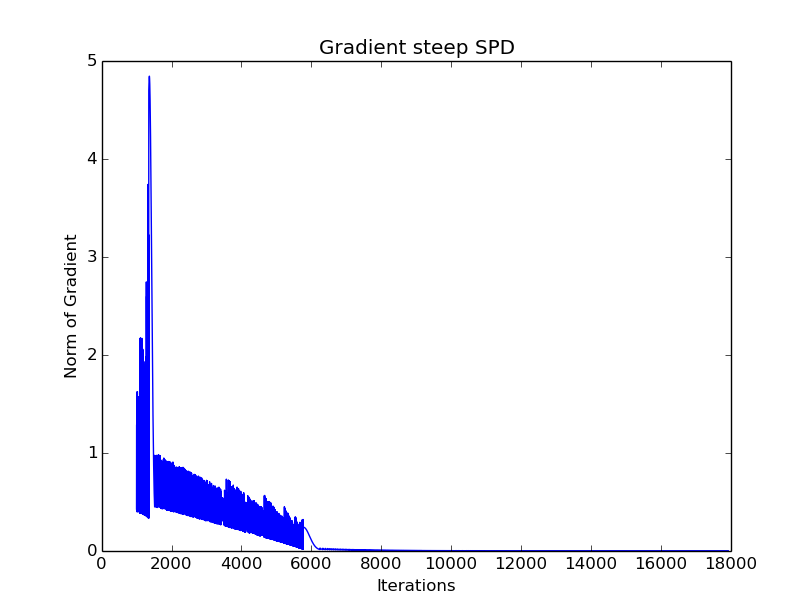
\includegraphics[scale=0.5]{steepspd.png}
  \caption{Gradient steep SPD}
\end{figure}
\begin{figure}[H]
  \centering
  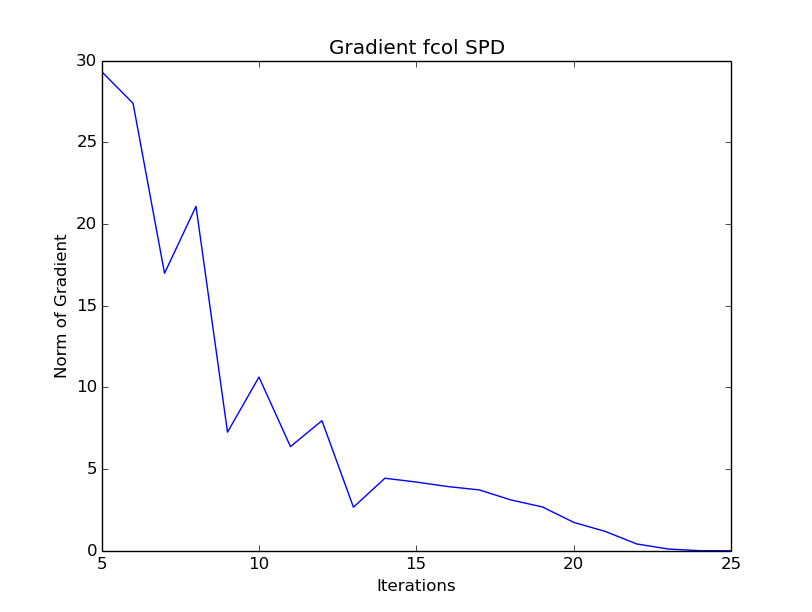
\includegraphics[scale=0.5]{fcolspd.png}
  \caption{Gradient fcol SPD}
\end{figure}
\begin{figure}[H]
  \centering
  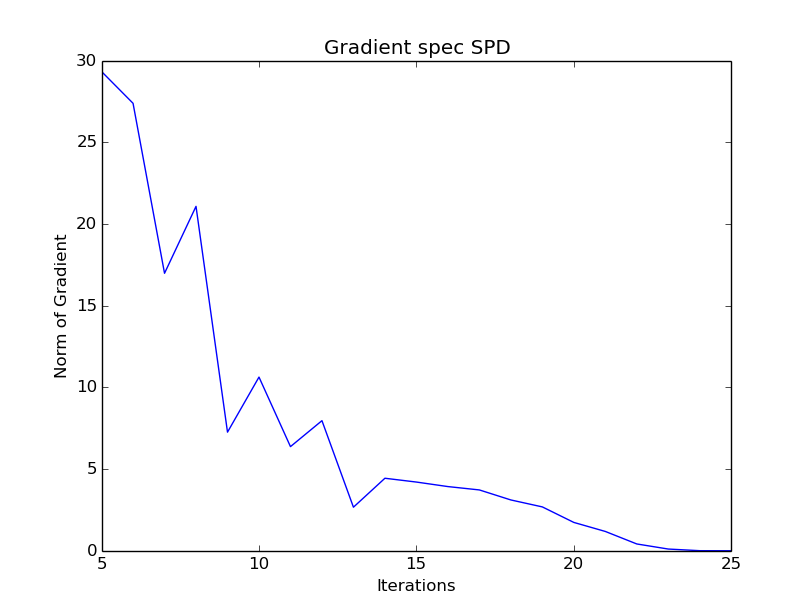
\includegraphics[scale=0.5]{specspd.png}
  \caption{Gradient spec SPD}
\end{figure}
\begin{figure}[H]
  \centering
  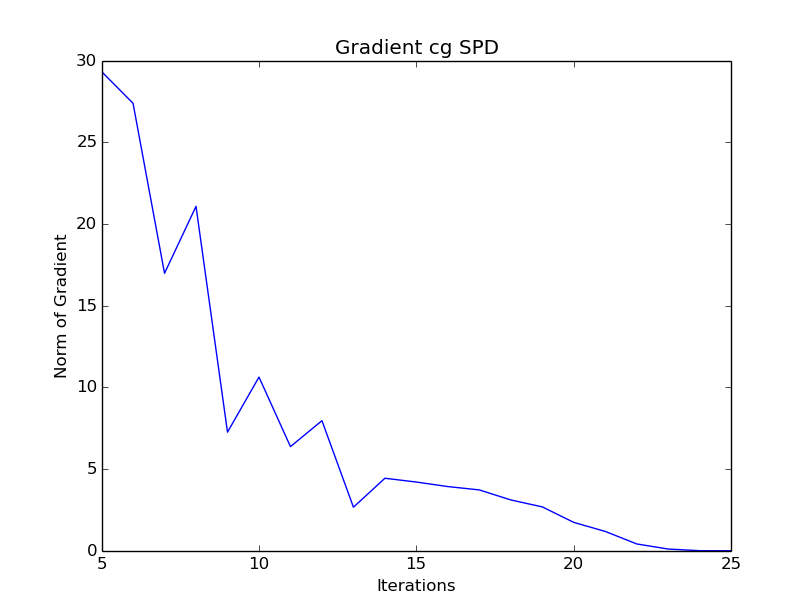
\includegraphics[scale=0.5]{cgspd.png}
  \caption{Gradient cg SPD}
\end{figure}
In this case, the figures support the conclusion of the last table, they show that the quasi-Newton methods perform
similarly and they clearly outperform steepest descent.
\subsection{Hessian not SPD}
We can see that the hessian of the Rosenbrock function at the point $(-0.3125,0.6875)$ is not positive
definite, as one eigenvalue is negative. The  table illustrates the performance
of the four methods with this starting point and the setup described above.
\begin{table}[H]
  \centering
  \begin{tabular}{|l|c|c|c|}
    \hline
   \textbf{Method} & \textbf{Iterations} & \textbf{Function Evaluations} &\textbf{Jacobian Evaluations} \\ \hline
   steep &13863 &165561 &13864 \\ \hline
   fcol &8 &26 &9 \\ \hline
   spec &9 &46 &10 \\ \hline
   cg &7 &23 &8 \\ \hline
 \textbf{Method} & \textbf{Hessian Evaluations} & \textbf{Matrix Factorizations} & \textbf{Multiplications with Hessian} \\ \hline
 steep &0 & 0 & 0 \\ \hline
   fcol &8 &13 &8 \\ \hline
   spec &9 &18 &9 \\ \hline
   cg &7 &0 &12 \\ \hline
  \end{tabular}
  \caption{Performance SPD}
  \label{tab:perform2}
\end{table}
As we can see from the values in the table, the quasi-Newton methods all perform similarly.
But, you can still notice that the biggest advantage of the conjugate gradient method is the fact that no
matrix factorizations are needed. On the downside, the number of matrix-vector multiplications is higher and we
will later see that region of convergence is smaller than the one of the other methods. The fcol method has the
smallest number of matrix vector multiplications but a higher number of matrix factorizations. The spec method
has as its biggest downside the higher number of factorization. This is due to fact that the matrix was factored to determine the eigenvalues and to solve the linear system of equations.
Note that this could be done (by not using cholfact to solve the system) with one factorization in the case when the hessian is SPD. Yet again, the performance of the steepest descent method is not competitive due to the slow convergence. \par
The figures illustrate how the norm of the gradient changes over the iterations.
\begin{figure}[H]
  \centering
  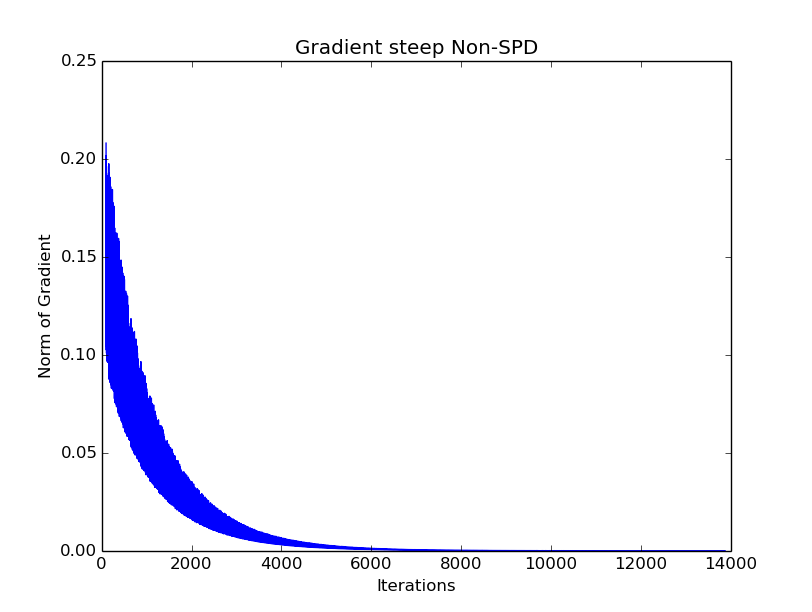
\includegraphics[scale=0.5]{steepnspd.png}
  \caption{Gradient steep Non-SPD}
\end{figure}
\begin{figure}[H]
  \centering
  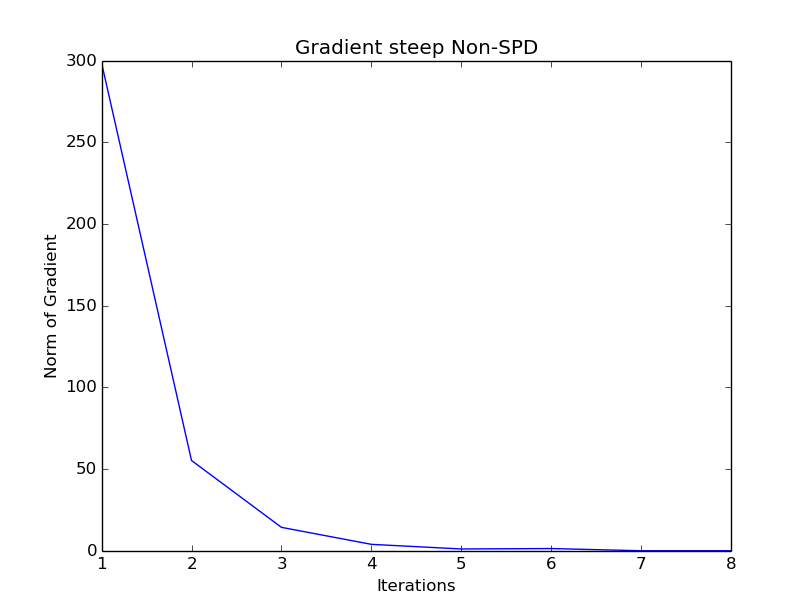
\includegraphics[scale=0.5]{fcolnspd.png}
  \caption{Gradient fcol Non-SPD}
\end{figure}
\begin{figure}[H]
  \centering
  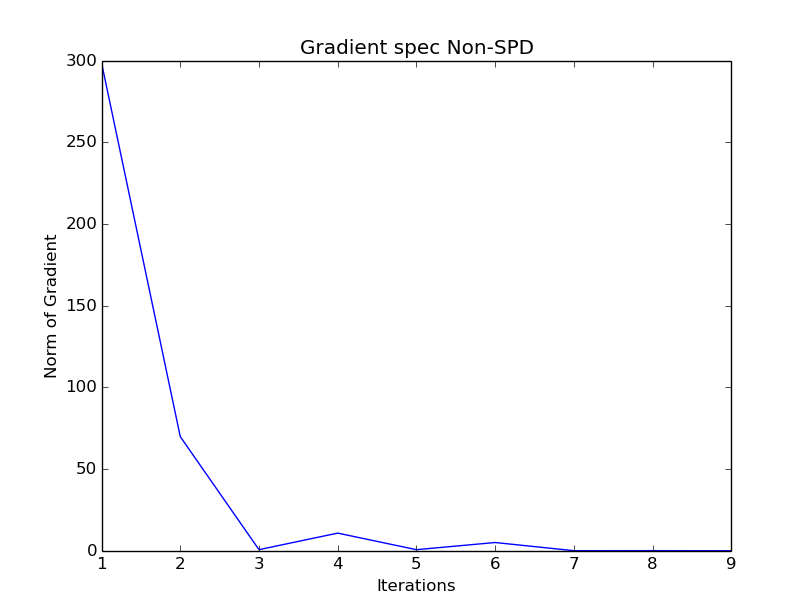
\includegraphics[scale=0.5]{specnspd.png}
  \caption{Gradient spec Non-SPD}
\end{figure}
\begin{figure}[H]
  \centering
  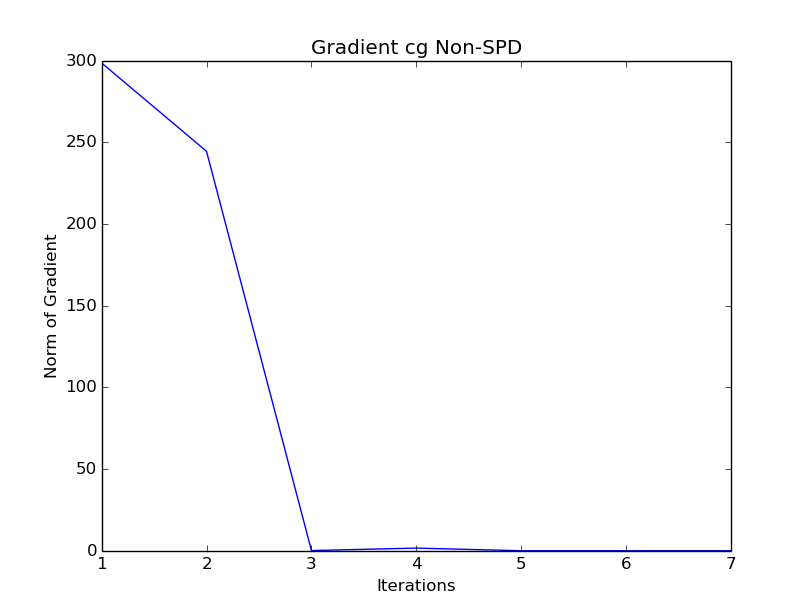
\includegraphics[scale=0.5]{cgnspd.png}
  \caption{Gradient cg Non-SPD}
\end{figure}
Yet again, the figures support the conclusion of the last table, they show that the quasi-Newton methods perform
similarly and they clearly outperform steepest descent.

\subsection{Region of Convergence}
The following plots illustrate the region of convergence.
In these plots, you can see the convergence in the region $[-2,2]\times [-1,3]$ by creating a $32\times 32$ equidistant mesh
on it.  The plot indicates the region and the numbering on the axis has to be understood relatively. The point $(3,4)$ 
is not representing the point $(3,4)$ in the cartesian plane but the corresponding point in the mesh. \par
All methods converge everywhere but cg. The region where it does not converge is white, while black represents convergence.
This is a strong disadvantage of this method especially considering that these points are relatively close to the solution.
\begin{figure}[H]
  \centering
  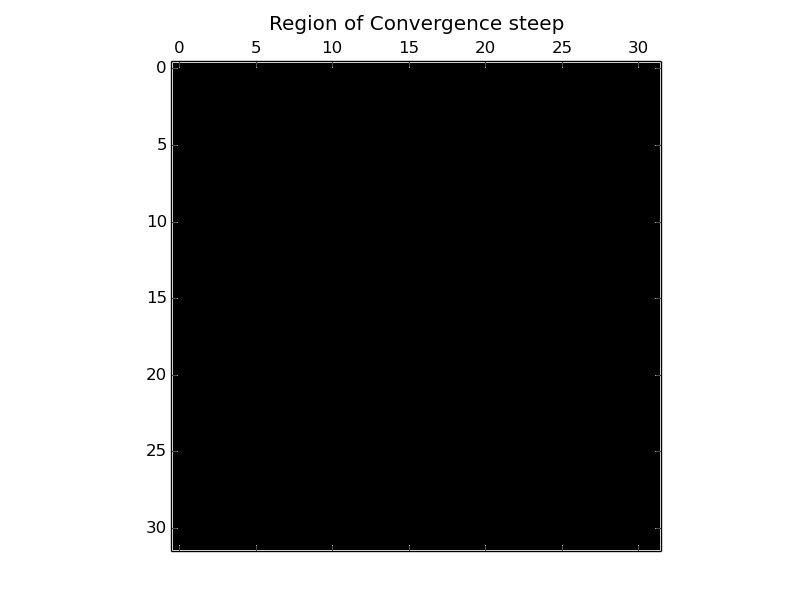
\includegraphics[scale=0.5]{steepregion.png}
  \caption{Gradient steep Non-SPD}
\end{figure}
\begin{figure}[H]
  \centering
  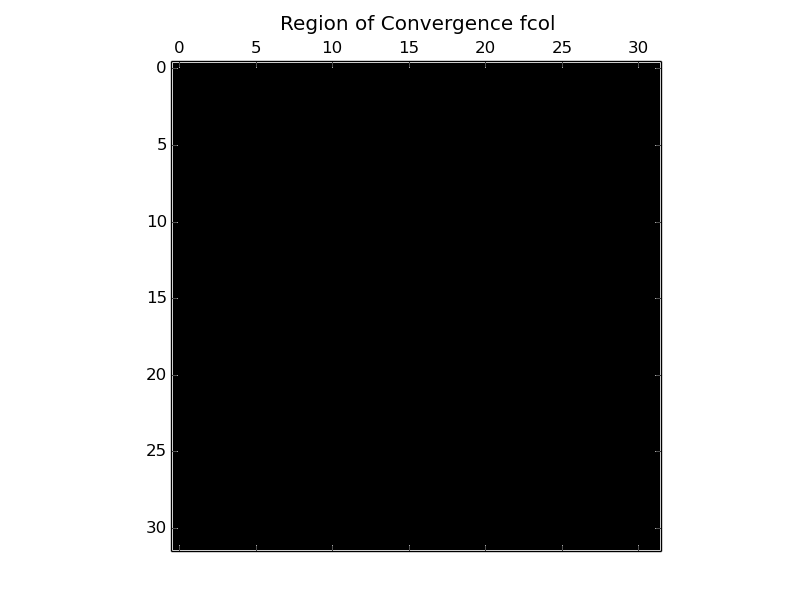
\includegraphics[scale=0.5]{fcolregion.png}
  \caption{Gradient fcol Non-SPD}
\end{figure}
\begin{figure}[H]
  \centering
  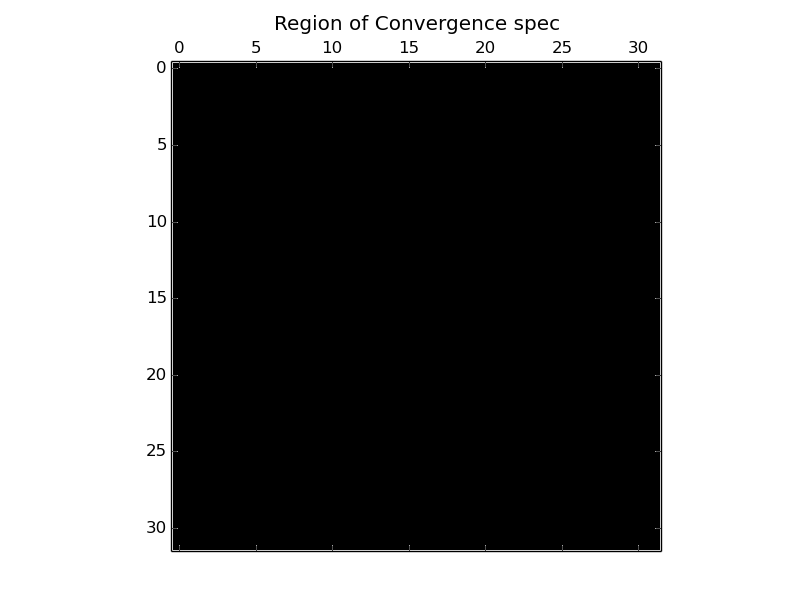
\includegraphics[scale=0.5]{specregion.png}
  \caption{Gradient spec Non-SPD}
\end{figure}
\begin{figure}[H]
  \centering
  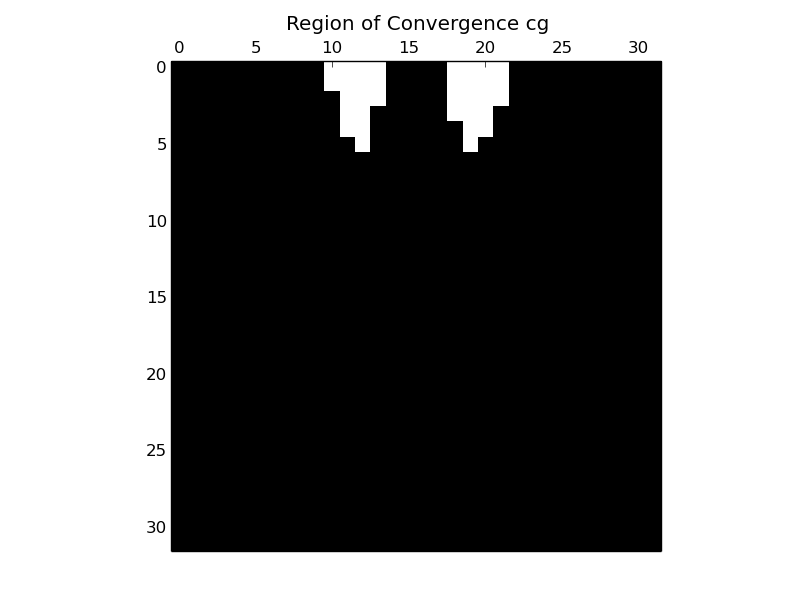
\includegraphics[scale=0.5]{cgregion.png}
  \caption{Gradient cg Non-SPD}
\end{figure}

\section{Exercise 2}
In this exercise we apply all four methods to the example from last homework. I will continue to use the notation from last
homework and not recall the details given there for the sake of brevity. In order to apply all methods, we first have to determine
the hessian. \par
The following plot indicates that the hessian that we determined is correct. Its formula is not relevant for further discussions so we do not
include it here.
\begin{figure}[H]
  \centering
  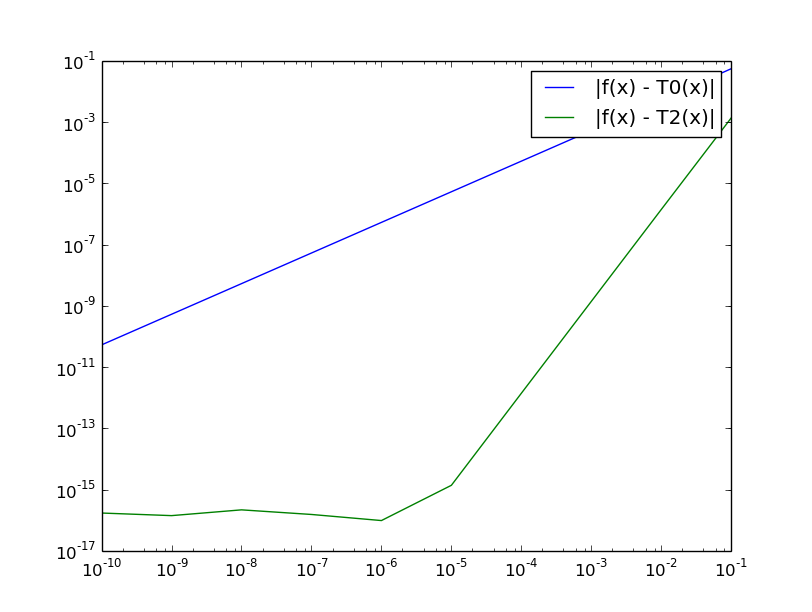
\includegraphics[scale=0.5]{hessian2.png}
  \caption{Check Hessian}
\end{figure}
We will now apply all four methods to the function where we have set $\alpha=2$ and $\beta=5$. The setup is identical to the one
in exercise 1. The hessian at our starting point is not spd, in fact exactly one of the 18 eigenvalues is negative.\par
The following table illustrates ones more that the convergence of steepest descent is not competitive. Furthermore,
fcol performs much weaker than the other two methods. Note that at our starting point, the matrix has only one negative eigenvalue and
17 positive ones. So, in some sense, it is close to being spd. It seems plausible that spec and cg can take advantage of this situation better as cg's approximation
of a solution will be accurate and spec modifies the matrix more efficiently than fcol in this case. The high number of matrix factorizations that fcol has to perform
supports this.
\begin{figure}
\begin{table}[H]
  \centering
  \begin{tabular}{|l|c|c|c|}
    \hline
   \textbf{Method} & \textbf{Iterations} & \textbf{Function Evaluations} &\textbf{Jacobian Evaluations} \\ \hline
   steep &331 &994 &332 \\ \hline
   fcol &17 &55 &18 \\ \hline
   spec &4 &17 &5 \\ \hline
   cg &5 &17 &6 \\ \hline
 \textbf{Method} & \textbf{Hessian Evaluations} & \textbf{Matrix Factorizations} & \textbf{Multiplications with Hessian} \\ \hline
 steep &0 & 0 & 0 \\ \hline
   fcol &17 &31 &17 \\ \hline
   spec &4 &8 &4 \\ \hline
   cg &5 &0 &45 \\ \hline
  \end{tabular}
  \caption{Performance SPD}
  \label{tab:perform3}
\end{table}
\end{figure}
The following plots show that all methods converge to the same solution.
\begin{figure}[H]
  \centering
  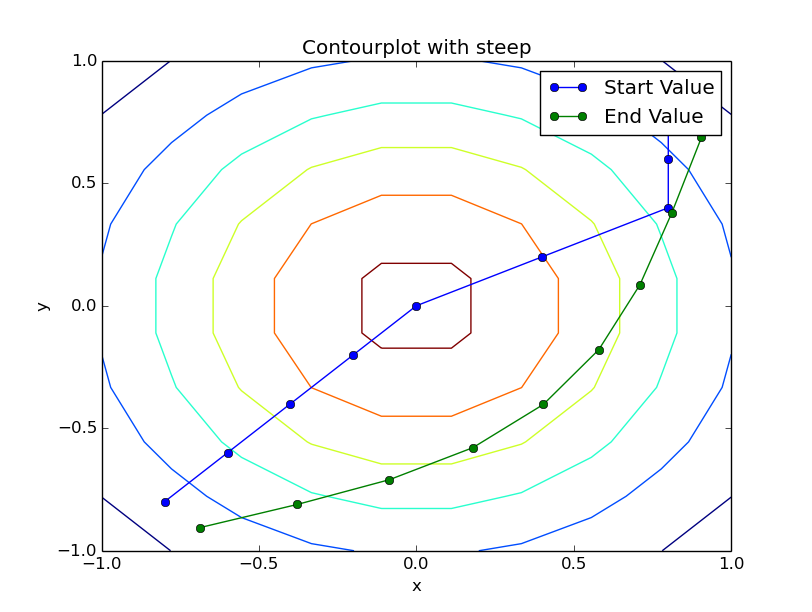
\includegraphics[scale=0.5]{2steep.png}
  \caption{Convergence steep}
\end{figure}
\begin{figure}[H]
  \centering
  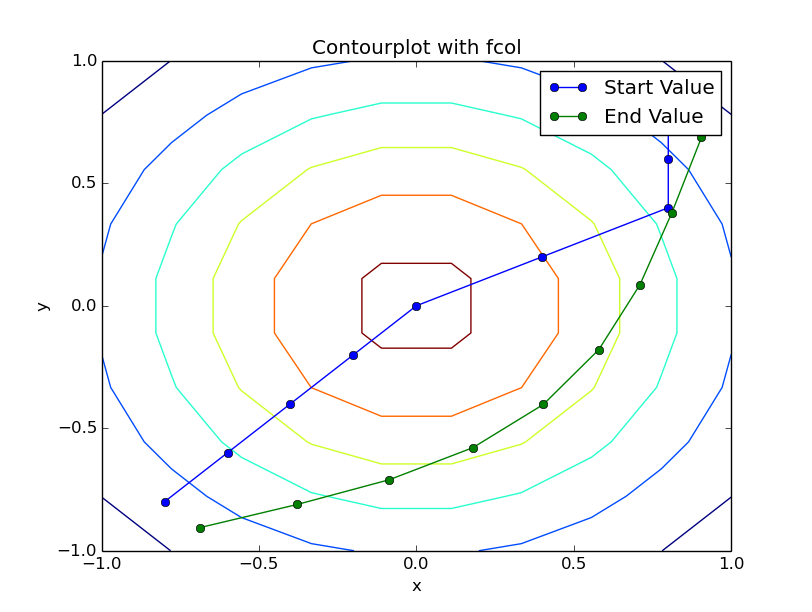
\includegraphics[scale=0.5]{2fcol.png}
  \caption{Convergence fcol}
\end{figure}
\begin{figure}[H]
  \centering
  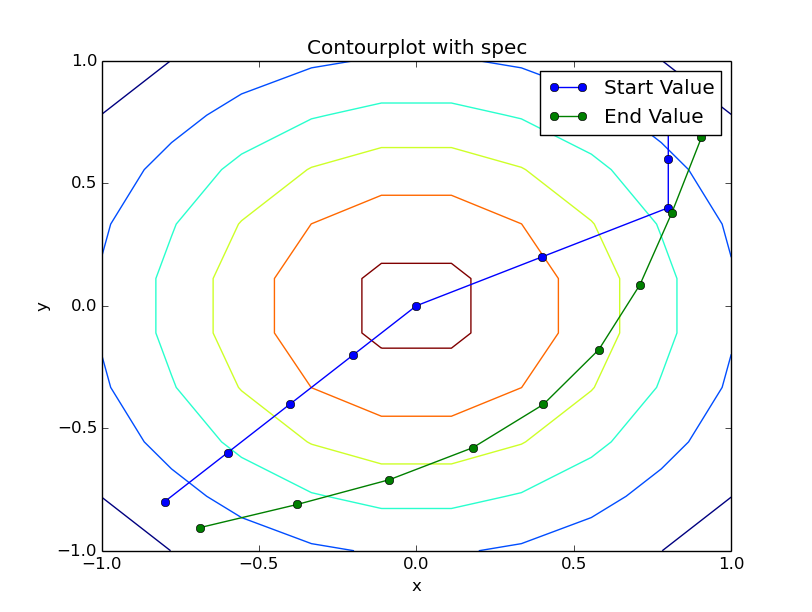
\includegraphics[scale=0.5]{2spec.png}
  \caption{Convergence spec}
\end{figure}
\begin{figure}[H]
  \centering
  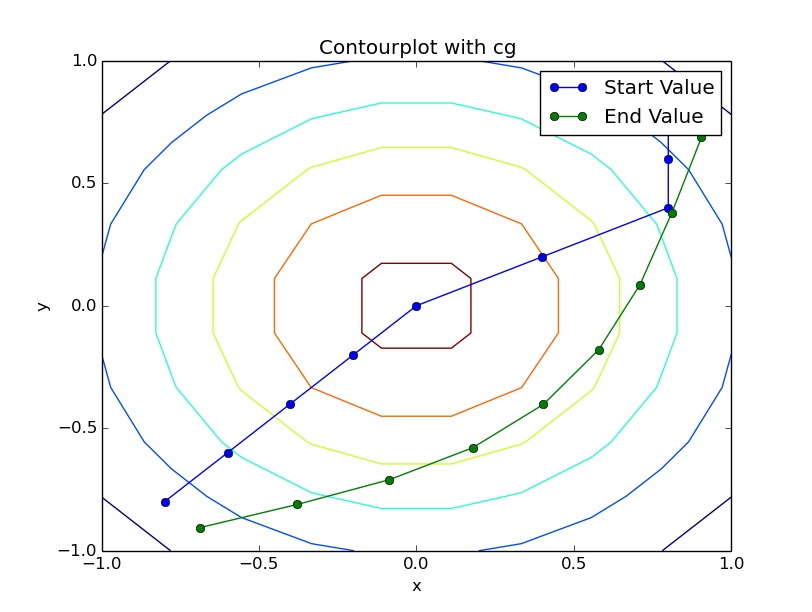
\includegraphics[scale=0.5]{2cg.png}
  \caption{Convergence cg}
\end{figure}
The following figures now show how the norm of the gradient changes over each iteration.
\begin{figure}[H]
  \centering
  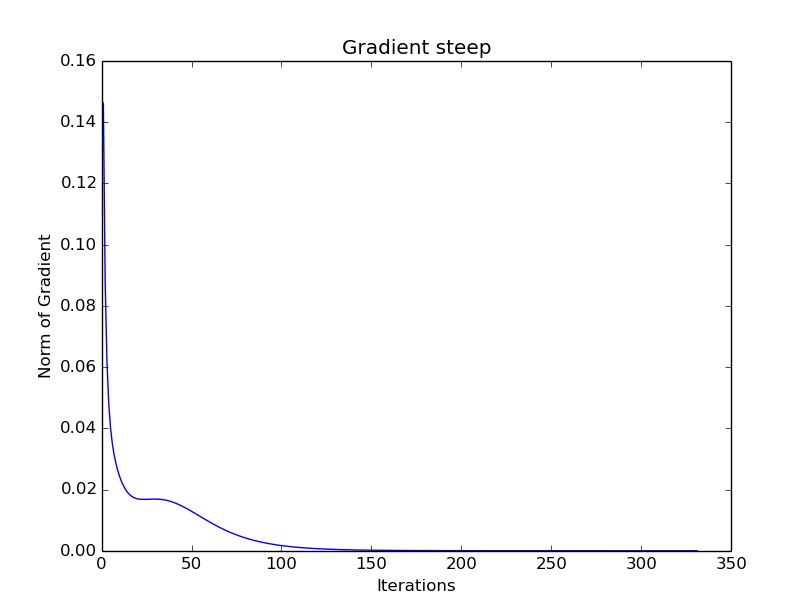
\includegraphics[scale=0.5]{3steep.png}
  \caption{Gradient steep}
\end{figure}
\begin{figure}[H]
  \centering
  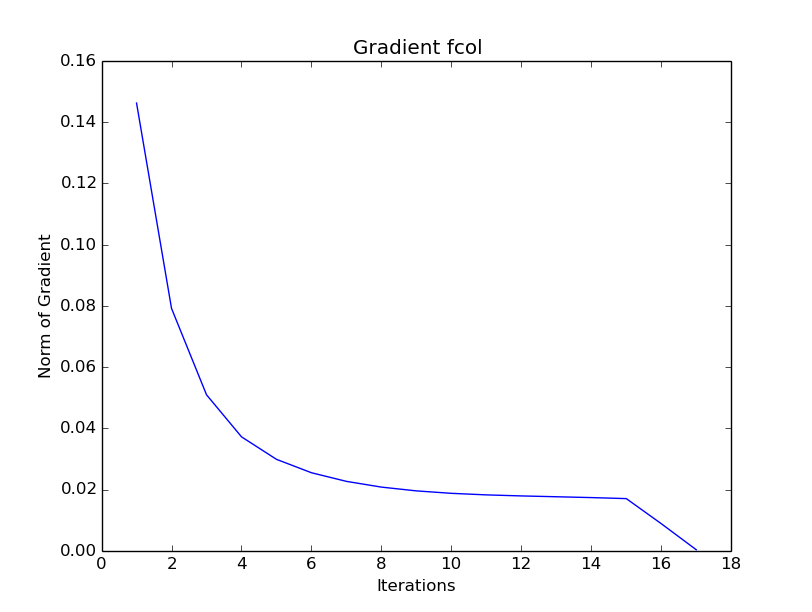
\includegraphics[scale=0.5]{3fcol.png}
  \caption{Gradient fcol}
\end{figure}
\begin{figure}[H]
  \centering
  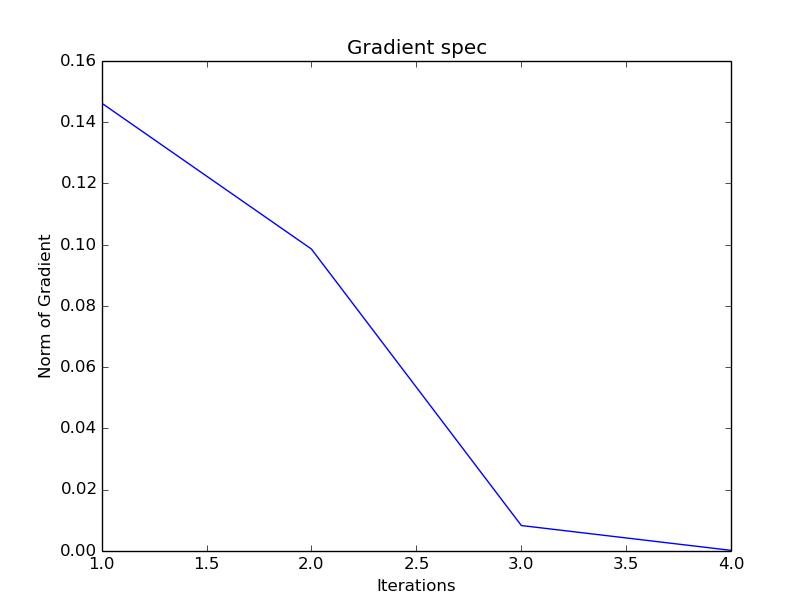
\includegraphics[scale=0.5]{3spec.png}
  \caption{Gradient spec}
\end{figure}
\begin{figure}[H]
  \centering
  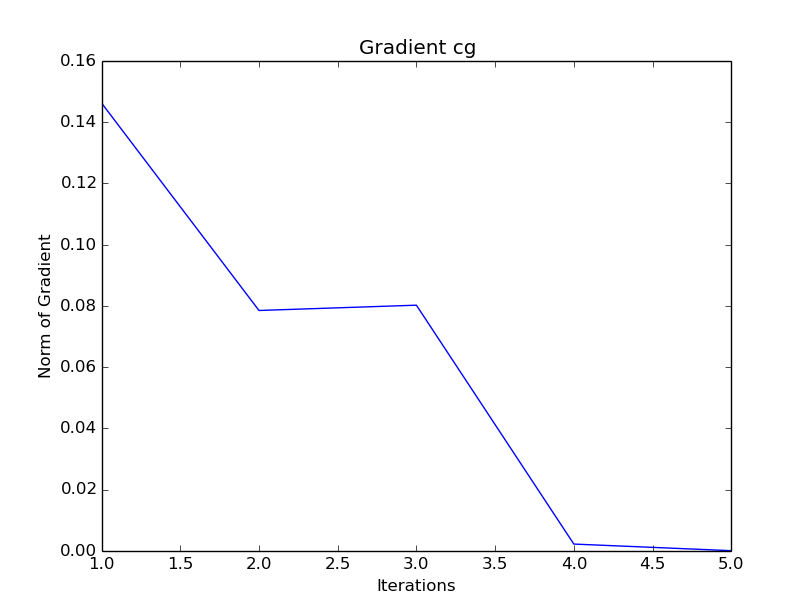
\includegraphics[scale=0.5]{3cg.png}
  \caption{Gradient cg}
\end{figure}
As the table and these figures suggest, all quasi-Newton methods are superior to the steepest descent method. In this particular example, the spec method seems to perform the best.
\end{document}